\chapter{Solución y marco teórico} % Título del capítulo. Lo agrega automaticamente al índice.
\label{cap:solucion} % etiqueta para las referencias a este capítulo
\markboth{Solución y marco teórico}{Solución y marco teórico} % Título que aparecerá en la cabecera de las siguientes páginas.
\vspace*{-2cm} % Reduce el espaciado, para que el párrafo este mas cerca del título.


% Solución propuesta (detalle).
% Marco teórico: Métodos, teorías y explicación, algoritmos, etc.

\section{Marco de desarrollo e implementación}

Para el desarrollo del proyecto, se decidió tomar como ejemplo un proyecto Open Source creado por Reiichiro Nakano disponibe en GitHub de nombre \href{https://github.com/reiinakano/arbitrary-image-stylization-tfjs}{\emph{``Arbitrary style transfer in TensorFlow.js''}} \cite{nakanoReiinakanoArbitraryimagestylizationtfjs2020}. Cuenta con una \href{https://reiinakano.com/arbitrary-image-stylization-tfjs/}{implementación demostrativa} de esta transferencia de estilos disponible en línea: \emph{https://reiinakano.com/arbitrary-image-stylization-tfjs/}\\
Este proyecto, implementa la transferencia de estilos (figura \ref{fig:stylize}) y además implementa una combinación de estilos para generar una imagen.



\begin{figure}[H]
  \includegraphics[scale=0.15]{img/mesa3/stylize}
  \centering
  %\vspace{-0.1cm}
  \caption{Arbitrary style transfer in TensorFlow.js: cambio de estilo}
  \label{fig:stylize}
\end{figure}

\clearpage


Para realizar esta transferencia de estilos, el creador de este proyecto se basó principalmente en las siguientes dos publicaciones:
\begin{itemize}
  \item ``Exploring the structure of a real-time, arbitrary neural artistic stylization network'', Ghiasi et. al. \cite{ghiasiExploringStructureRealtime2017}
  \item ``Distilling the Knowledge in a Neural Network'', Hinton et. al. \cite{hintonDistillingKnowledgeNeural2015}
\end{itemize}

En ``Exploring the structure of a real-time, arbitrary neural artistic stylization network'', Ghiasi et. al. \cite{ghiasiExploringStructureRealtime2017} se expone una arquitectura para la transferencia de estilos para una \emph{imagen que aporta el contenido y otra que aporta el estilo}.
\begin{itemize}
  \item \textbf{Imagen de contenido}, es la imagen que se quiere generar con otro estilo.
  \item \textbf{Imagen de estilo}, es la imagen que aporta el estilo, y por lo tanto, es el estilo que se quiere transferir a \emph{imagen de contenido}.
\end{itemize}


Para ello se definen dos redes neuronales, una \emph{red de transferencia de estilo} (style transfer network) y una \emph{red de predicción de estilo} (style prediction network), tal como se muestra en la Figura \ref{fig:arquitectura}.

\begin{itemize}
  \item \textbf{Style transfer network:} la red de transferencia de estilo, toma un set de parámetros representativos del estilo y la imagen que aporta el contenido, y genera la imagen que aporta contenido estilizada.
  \item \textbf{Style prediction network:} la red de predicción de estilo genera para cada \emph{imagen de estilo} un set de parámetros representativos, que después serán utilizados para proveer a la \emph{style transfer network} con los parámetros necesarios para generar la imagen estilizada.
\end{itemize}

\begin{figure}[H]
  \includegraphics[scale=0.3]{img/mesa3/p2}
  \centering
  %\vspace{-0.1cm}
  \caption{Arquitectura para transferencia de estilos implementada}
  \label{fig:arquitectura}
  \end{figure}




Con el objetivo de portar estos modelos a TensorFlow.js de una forma más eficiente,
se usó una técnica
llamada destilación (Distillation) propuesta en ``Distilling the Knowledge in a Neural Network'', Hinton et. al. \cite{hintonDistillingKnowledgeNeural2015}.
Esta técnica consiste básicamente en comprimir el ``conocimiento'' interno de una red neuronal de mayor tamaño y embebirlo en una red de menor tamaño.\\
De esta forma, se toma una red neuronal más pequeña para replicar de forma directa las salidas de la red de mayor tamaño. En este caso, se comprimió un modelo Inception V3 en un modelo MobileNet V2.
Este proceso de acuerdo a la figura \ref{fig:destilacion}, consiste en tomar la \emph{imagen de estilo} y pasarla a través del modelo Inception V3 y MobileNet V2, obteniendo de esta forma 2 \emph{set de parámetros representativos} para cada imagen. Después de esto, se toma como función de pérdida (loss function) el
error cuadrático medio (MSE, Mean Square Error) entre estos 2 set de parámetros representativos, y se usa para actualizar los pesos de MobileNet V2.\\
El código para realizar esta destilación entre estos modelos está disponible en el \href{https://github.com/magenta/magenta/tree/master/magenta/models/arbitrary_image_stylization}{repositorio de Git Hub del proyecto Magenta para transferencia de estilos}.\\


Se debe mencionar que el modelo MobileNet V2 tiene una implementación Open Source disponible en python y ha sido portado a TensorFlow.js:
\begin{itemize}
  \item Implementación en python: \href{https://github.com/tensorflow/models/tree/master/research/slim/nets/mobilenet}{Repositorio TensorFlow Models}

  \item Implementación portada a TensorFlow.js: \href{https://github.com/tensorflow/tfjs-examples/tree/master/mobilenet}{Repositorio de ejemplos de TensorFlow.js}
\end{itemize}

\begin{figure}[H]
  \includegraphics[scale=0.3]{img/mesa3/p1}
  \centering
  %\vspace{-0.1cm}
  \caption{Proceso de entrenamiento: Destilación (Distillation \cite{hintonDistillingKnowledgeNeural2015}) }
  \label{fig:destilacion}
\end{figure}





%%%%%%%%%%%%%%%%%%%%%%%%%%%%%%%%%%%%%%%%%%%%%%%%%%%%%%%%%%%%%%%%%%%%%%%%%%%%%%%%%%%%%%%%%%%%%%%%%%%%%%%%
%%%%%%%%%%%%%%%%%%%%%%%%%%%%%%%%%%%%%%%%%%%%%%%%%%%%%%%%%%%%%%%%%%%%%%%%%%%%%%%%%%%%%%%%%%%%%%%%%%%%%%%%
%%%%%%%%%%%%%%%%%%%%%%%%%%%%%%%%%%%%%%%%%%%%%%%%%%%%%%%%%%%%%%%%%%%%%%%%%%%%%%%%%%%%%%%%%%%%%%%%%%%%%%%%
%%%%%%%%%%%%%%%%%%%%%%%%%%%%%%%%%%%%%%%%%%%%%%%%%%%%%%%%%%%%%%%%%%%%%%%%%%%%%%%%%%%%%%%%%%%%%%%%%%%%%%%%
%%%%%%%%%%%%%%%%%%%%%%%%%%%%%%%%%%%%%%%%%%%%%%%%%%%%%%%%%%%%%%%%%%%%%%%%%%%%%%%%%%%%%%%%%%%%%%%%%%%%%%%%
%%%%%%%%%%%%%%%%%%%%%%%%%%%%%%%%%%%%%%%%%%%%%%%%%%%%%%%%%%%%%%%%%%%%%%%%%%%%%%%%%%%%%%%%%%%%%%%%%%%%%%%%
%%%%%%%%%%%%%%%%%%%%%%%%%%%%%%%%%%%%%%%%%%%%%%%%%%%%%%%%%%%%%%%%%%%%%%%%%%%%%%%%%%%%%%%%%%%%%%%%%%%%%%%%
%%%%%%%%%%%%%%%%%%%%%%%%%%%%%%%%%%%%%%%%%%%%%%%%%%%%%%%%%%%%%%%%%%%%%%%%%%%%%%%%%%%%%%%%%%%%%%%%%%%%%%%%




\clearpage
\subsection{Implementación}










Para el desarrollo de la plataforma, se optó por reutilizar parte del código del proyecto
\href{https://github.com/reiinakano/arbitrary-image-stylization-tfjs}{\emph{``Arbitrary style transfer in TensorFlow.js''}} \cite{nakanoReiinakanoArbitraryimagestylizationtfjs2020}, y rescatar las ideas básicas de su implementación para posteriormente realizar un implementación completamente nueva. Ejemplo de esto es el código en Listado \ref{codMod} que implementa una función asíncrona genérica  para cargar un modelo preentrenado para su posterior ejecución.

\lstset{style=customjs}
\begin{center}
\begin{minipage}{0.78\linewidth}
%\label{lst:codMod}
\begin{lstlisting}[caption=Código en JavaScript para cargar modelos, label=codMod]
  async loadMobileNetStyleModel() {
    if (!this.mobileStyleNet) {
      this.mobileStyleNet = await tf.loadGraphModel(
        'saved_model_style_js/model.json');
    }

    return this.mobileStyleNet;
  }
\end{lstlisting}
\end{minipage}
\end{center}




\subsubsection{Marco de desarrollo y trabajo}

El marco de desarrollo y trabajo se define como la forma básica y principal de utilización y trabajo en la plataforma. Este debe tener en cuenta la forma de trabajo con los lenguajes de programación y librerías implicadas. \\
De esta forma, el proceso descrito a continuación puede tomarse como la forma básica de trabajo para la implementación de modelos con TensorFlow.js .

\textbf{Descripción del proceso:}
\vspace{-0.4cm}
\begin{enumerate}
  \item Diseño y entrenamiento del modelo en lenguaje Python, utilizando la API TensorFlow.
  \item Guardado del modelo en un tipo compatible con \href{https://github.com/tensorflow/tfjs/tree/master/tfjs-converter}{\emph{convertidor de modelos}} \cite{TensorflowTfjs}.
  \item Conversion del modelo a formato web compatible, utilizando \href{https://github.com/tensorflow/tfjs/tree/master/tfjs-converter}{\emph{convertidor de modelos}}.
  \item Implementación del modelo en TensorFlow.js .
\end{enumerate}

\vspace{-0.2cm}
De esta forma de acuerdo a lo anterior, resumido en la Figura \ref{fig:proceso}:
\vspace{-0.4cm}
\begin{itemize}
  \item Los puntos 1,2 y 3, pueden conseguirse con la inclusión en el código de entrenamiento y/o diseño en Python del template en Listado \ref{codConv}.
  \begin{itemize}
    \item Línea 1, importa TensorFlow.js
    \item Línea 5-7, guarda el modelo entrenado en formato .h5
    \item Línea 8, llama al convertidor de modelos, declara el formato de entrada como \emph{keras} (en el caso de haber hecho uso de esta API), le entrega el directorio de guardado como \emph{saved\_model\_path}, y declara el directorio de guardado del modelo convertido como \emph{./} (directorio actual de ejecución).
  \end{itemize}
\end{itemize}



\begin{figure}[H]
  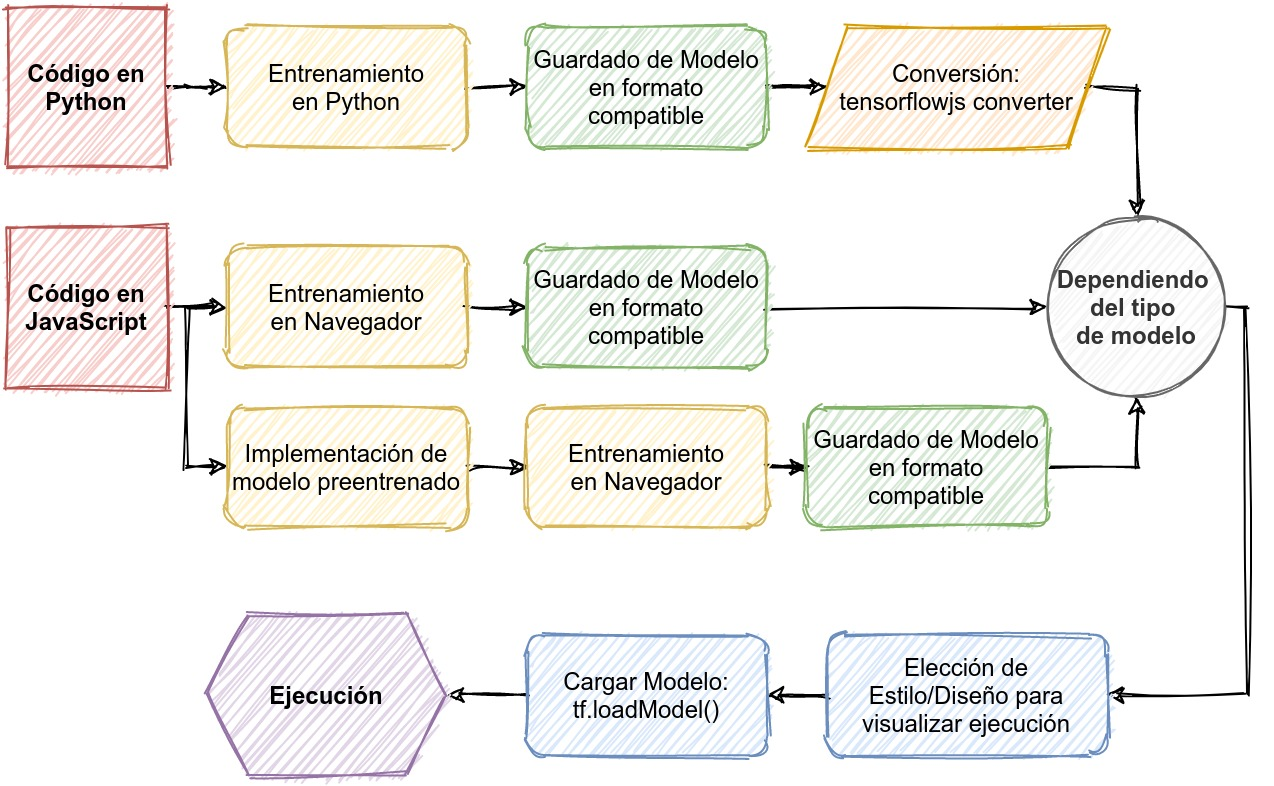
\includegraphics[scale=0.6]{img/fix0/diag_flujo}
  \centering
  %\vspace{-0.1cm}
  \caption{Proceso básico de desarrollo}
  \label{fig:proceso}
\end{figure}


\begin{center}
  %\begin{minipage}{0.78\linewidth}
  \lstset{style=custom_python}
  %\label{lst:codConv}
  \begin{lstlisting}[caption=Código base en Python para convertir modelos, label=codConv]
    !pip install tensorflowjs

    [CODIGO PYTHON]

    import time
    saved_model_path = "./{}.h5".format(int(time.time()))
    model.save(saved_model_path)
    !tensorflowjs_converter --input_format=keras {saved_model_path} ./
  \end{lstlisting}
  %\end{minipage}
  \end{center}












%%%%%%%%%%%%%%%%%%%%%%%%%%%%%%%%%%%%%%%%%%%%%%%%%%%%%%%%%%%%%%%%%%%%%%%%%%%%%%%%%%%%%%%%%%%%%%%%%%%%%%%%
%%%%%%%%%%%%%%%%%%%%%%%%%%%%%%%%%%%%%%%%%%%%%%%%%%%%%%%%%%%%%%%%%%%%%%%%%%%%%%%%%%%%%%%%%%%%%%%%%%%%%%%%
%%%%%%%%%%%%%%%%%%%%%%%%%%%%%%%%%%%%%%%%%%%%%%%%%%%%%%%%%%%%%%%%%%%%%%%%%%%%%%%%%%%%%%%%%%%%%%%%%%%%%%%%
%%%%%%%%%%%%%%%%%%%%%%%%%%%%%%%%%%%%%%%%%%%%%%%%%%%%%%%%%%%%%%%%%%%%%%%%%%%%%%%%%%%%%%%%%%%%%%%%%%%%%%%%
%%%%%%%%%%%%%%%%%%%%%%%%%%%%%%%%%%%%%%%%%%%%%%%%%%%%%%%%%%%%%%%%%%%%%%%%%%%%%%%%%%%%%%%%%%%%%%%%%%%%%%%%
%%%%%%%%%%%%%%%%%%%%%%%%%%%%%%%%%%%%%%%%%%%%%%%%%%%%%%%%%%%%%%%%%%%%%%%%%%%%%%%%%%%%%%%%%%%%%%%%%%%%%%%%
%%%%%%%%%%%%%%%%%%%%%%%%%%%%%%%%%%%%%%%%%%%%%%%%%%%%%%%%%%%%%%%%%%%%%%%%%%%%%%%%%%%%%%%%%%%%%%%%%%%%%%%%
%%%%%%%%%%%%%%%%%%%%%%%%%%%%%%%%%%%%%%%%%%%%%%%%%%%%%%%%%%%%%%%%%%%%%%%%%%%%%%%%%%%%%%%%%%%%%%%%%%%%%%%%



\clearpage
\subsection{Diseño base de plataforma}

Como una primera etapa en la implementación, se propone un diseño basado en el mismo proyecto base, pero haciendolo extensivo para su reutilización en la implementación de otros modelos. De esta forma, el diseño base se muestra en Figura \ref{fig:diseno1}.

\begin{figure}[H]
    \includegraphics[scale=0.4]{img/mesa3/d1}
    \centering
    %\vspace{-0.1cm}
    \caption{Diseño interfaz modelo tipo}
    \label{fig:diseno1}
\end{figure}

De acuerdo a la Figura \ref{fig:diseno1}, el diseño básico demarcado consta de 4 partes. Un título de la página, una selección para el \emph{modelo}, una zona relacionada propiamente con el modelo llamada ``Marco de predicción'' y una última zona relacionada con la descripción de nombre ``Marco de descripción''.
Se definen por lo tanto, lo siguiente:
\begin{itemize}
  \item \textbf{Título de la página:}
  zona de demarcación para título propio de la pagina en cuestion.
  Por motivos de descripción y facilidad de navegación,
  debe de disponer
  mínimamente de un títulos principal correspondiente al título general de la página y un subtítulo propio del modelo seleccionado relacionado con algún modelo en la zona de demarcación \emph{Selección de modelo}.\\

  \item \textbf{Selección de modelo:}
  zona de demarcación para la selección del modelo a utilizar.
  Esta zona está subdividida conforme a la cantidad de modelos implementados.\\

  \item \textbf{Marco de predicción:}
  zona que demarca el lugar en donde el modelo al ejecutarse muestra elresultado de su ejecución.
  Esta zona depende estrictamente del tipo de modelo a implementar, y por lo tanto, se definen como base dos tipos de modelos, \emph{Modelo tipo 1} y \emph{Modelo tipo 2}.\\

  \item \textbf{Marco de descripción:}
  es la zona en la cual el modelo seleccionado e implementado
  lleva una explicación propia de su funcionamiento. Esta explicación debe de contar con una explicación del funcionamiento del modelo a alto nivel mediante diagramas de bloques, y una explicación a más bajo nivel a nivel de código para comprender mejor su implementación. Citas y referencias deben acompañar esta descripción del modelo.

\end{itemize}


\clearpage
De esta forma, como una primera instancia y simplificación de la plataforma, se propone la implementación de acuerdo a dos tipos de modelos bases:
\begin{itemize}
  \item \textbf{Modelo tipo 1:} de acuerdo a Figura \ref{fig:diseno2}, diseño útil para la implementación de modelos en el que el resultado de su ejecución es principalmente una imagen, como es el caso de la implementación de un modelo de transferencia de estilos. De acuerdo a esto, es un diseño apto para modelos tales como:
  \begin{itemize}
    \item \href{https://github.com/tensorflow/tfjs-models/tree/master/posenet}{Estimación en tiempo real de posición del cuerpo con PoseNet}.
    \item \href{https://github.com/justadudewhohacks/face-api.js}{Detección y reconomiento de rostros con Face API}. \\
  \end{itemize}


  \item \textbf{Modelo tipo 2:} de acuerdo a Figura \ref{fig:diseno3}, diseño útil para la implementación de modelos en el que el resultado de su ejecución es principalmente texto. De acuerdo a esto, es un diseño apto para modelos tales como:
  \begin{itemize}
    \item \href{https://github.com/tensorflow/tfjs-models/tree/master/mobilenet}{Clasificación de imagenes con MobileNet}.
    \item \href{https://github.com/tensorflow/tfjs-models/tree/master/toxicity}{Clasificación de toxicidad de texto}.\\
  \end{itemize}

\end{itemize}

\begin{figure}[H]
  \includegraphics[scale=0.4]{img/mesa3/d2}
  \centering
  %\vspace{-0.1cm}
  \caption{Diseño interfaz modelo: tipo 1}
  \label{fig:diseno2}
\end{figure}

\begin{figure}[H]
  \includegraphics[scale=0.4]{img/mesa3/d3}
  \centering
  %\vspace{-0.1cm}
  \caption{Diseño interfaz modelo: tipo 2}
  \label{fig:diseno3}
\end{figure}

\clearpage
\subsection{Herramientas para el desarrollo}

De acuerdo a la implementación base, y teniendo en consideración la facilidad de implementación, programación y posterior claridad de uso, las herramientas de desarrollo utilizadas se pueden resumir en las siguientes: HTML, JavaScript, TensorFlow.js

\begin{itemize}
  \item HTML, para generar la estructura de la página web.
  \item CSS, como herramienta para inserción de estilos y orden en la estructura.
  \item JavaScript, como lenguaje de programación para describir los procedimientos y acciones, e implementación de TensorFlow.js.
\end{itemize}



Las principales herramientas de desarrollo a utilizar para esta implementación se listan a continuación:

\begin{itemize}
  \item \textbf{VS Code:} editor de texto desarrollado por Microsoft, open source, con gran cantidad de herramientas y extensiones, con implementación nativa de autocompletado de código en JavaScript.
  \item \textbf{Git:} herramienta para control de versiones y seguimiento en el desarrollo.
  \item \textbf{Git Hub:} servicio en la nube que implementa Git para el control de versiones, permitiendo de esta manera tener un respaldo del código en toda su fase de desarrollo e implementación, y con capacidad de servir sitios web de forma estática directamente desde un repositorio de código.
\end{itemize}





%%%%%%%%%%%%%%%%%%%%%%%%%%%%%%%%%%%%%%%%%%%%%%%%%%%%%%%%%%%%%%%%%%%%%%%%%%%%%%%%%%%%%%%%%%%%%%%%%%%%%%%%
%%%%%%%%%%%%%%%%%%%%%%%%%%%%%%%%%%%%%%%%%%%%%%%%%%%%%%%%%%%%%%%%%%%%%%%%%%%%%%%%%%%%%%%%%%%%%%%%%%%%%%%%
%%%%%%%%%%%%%%%%%%%%%%%%%%%%%%%%%%%%%%%%%%%%%%%%%%%%%%%%%%%%%%%%%%%%%%%%%%%%%%%%%%%%%%%%%%%%%%%%%%%%%%%%
%%%%%%%%%%%%%%%%%%%%%%%%%%%%%%%%%%%%%%%%%%%%%%%%%%%%%%%%%%%%%%%%%%%%%%%%%%%%%%%%%%%%%%%%%%%%%%%%%%%%%%%%
%%%%%%%%%%%%%%%%%%%%%%%%%%%%%%%%%%%%%%%%%%%%%%%%%%%%%%%%%%%%%%%%%%%%%%%%%%%%%%%%%%%%%%%%%%%%%%%%%%%%%%%%
%%%%%%%%%%%%%%%%%%%%%%%%%%%%%%%%%%%%%%%%%%%%%%%%%%%%%%%%%%%%%%%%%%%%%%%%%%%%%%%%%%%%%%%%%%%%%%%%%%%%%%%%
%%%%%%%%%%%%%%%%%%%%%%%%%%%%%%%%%%%%%%%%%%%%%%%%%%%%%%%%%%%%%%%%%%%%%%%%%%%%%%%%%%%%%%%%%%%%%%%%%%%%%%%%
%%%%%%%%%%%%%%%%%%%%%%%%%%%%%%%%%%%%%%%%%%%%%%%%%%%%%%%%%%%%%%%%%%%%%%%%%%%%%%%%%%%%%%%%%%%%%%%%%%%%%%%%



\clearpage
\subsection{Implementación base de plataforma}
De acuerdo a lo anterior, se implementa una primera plataforma online con base en las siguientes características:
\begin{itemize}
  \item Se genera un repositorio en GitHub, ordenando archivos para mayor claridad.
  \begin{itemize}
    \item \textbf{Repositorio:} \url{https://github.com/ccofres/ccofres.github.io/tree/gh-pages}
  \end{itemize}
  \item Se genera sitio web de forma automática por GitHub Pages desde el repositorio.
  \item Bajo la carpeta \textbf{Modelos} pueden ser agregadas nuevas implementaciones, para posteriormente ser agregados al menú editando directamente el documento \emph{model.html}.
\end{itemize}

\begin{figure}[H]
  \includegraphics[scale=0.4]{img/fix0/gh1}
  \includegraphics[scale=0.4]{img/fix0/gh2}
  \centering
  %\vspace{-0.1cm}
  \caption{Estructura de archivos en GitHub}
  \label{fig:gh-pages}
\end{figure}

De esta forma, es posible clonar o descargar de forma local el proyecto, y utilizar estos modelos a través de la generación de un servidor web local a través
de las \textbf{Chrome Apps} en el navegador Google Chrome:
\begin{itemize}
  \item Las Chrome Apps están disponibles en \url{chrome://apps/}
  \begin{figure}[H]
    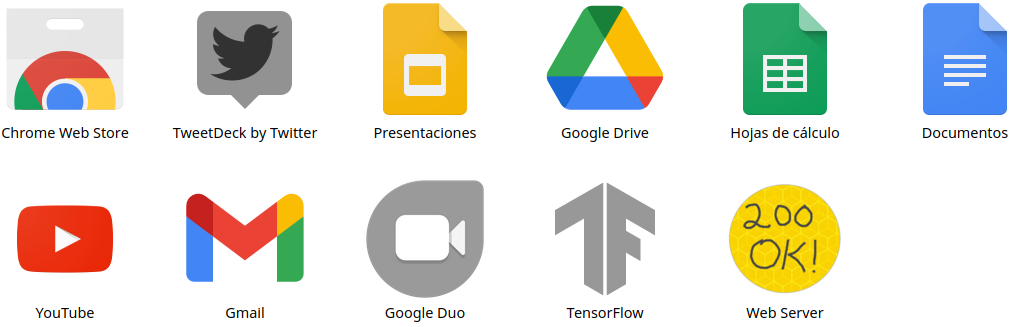
\includegraphics[scale=0.15]{img/fix0/chrome-apps}
    \centering
    %\vspace{-0.1cm}
    \caption{Chrome Apps de Google Chrome}
    \label{fig:chrome-apps}
  \end{figure}

  \begin{figure}[H]
    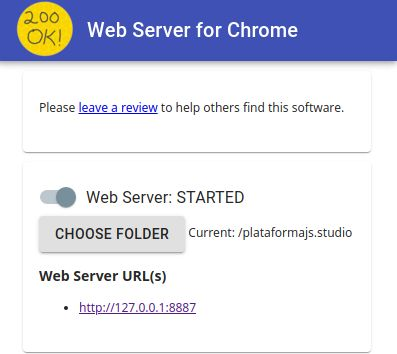
\includegraphics[scale=0.3]{img/fix0/chrome-apps2}
    \centering
    %\vspace{-0.1cm}
    \caption{Servidor local generado en base a la carpeta del proyecto }
    \label{fig:chrome-apps2}
  \end{figure}
\end{itemize}
Parte de los modelos en JavaScript implementados quedan disponibles en Apéndice \ref{cap:unApendice}.
Esta plataforma, aún en desarrollo, toma por nombre \emph{Plataforma JS} y está disponible en el dominio \url{https://plataformajs.studio/}.